\PassOptionsToPackage{hyperfootnotes=false}{hyperref}
\documentclass[fleqn,usenatbib]{mnras}
\usepackage[T1]{fontenc}
\usepackage{graphicx}
\usepackage{amsmath,amssymb}
\usepackage{booktabs}
\usepackage{array}
\usepackage{float}
\usepackage[section]{placeins}
\usepackage{microtype}
\usepackage{hyperref}
\usepackage{subcaption}
\usepackage{balance}
\hypersetup{hidelinks}
\clubpenalty=10000
\widowpenalty=10000
\displaywidowpenalty=10000
\setlength{\textfloatsep}{10pt plus 2pt minus 2pt}
\setlength{\floatsep}{8pt plus 2pt minus 2pt}
\setlength{\intextsep}{8pt plus 2pt minus 2pt}
\setlength{\dbltextfloatsep}{10pt plus 2pt minus 2pt}
\setlength{\dblfloatsep}{8pt plus 2pt minus 2pt}
\setlength{\abovecaptionskip}{4pt}
\setlength{\belowcaptionskip}{2pt}

\title[A reproducible earned-versus-enforced benchmark for dynamic VLBI]{A reproducible earned-versus-enforced benchmark for dynamic VLBI}
\author[Zacharioudakis]{Stylianos Georgios Zacharioudakis$^{1}$\thanks{E-mail: sdi2200243@di.uoa.gr}\\
$^{1}$\parbox[t]{0.84\textwidth}{Department of Informatics and Telecommunications, National and Kapodistrian University of Athens, Panepistimioupolis, Athens 16122, Greece}}
\date{Accepted XXX. Received YYY; in original form ZZZ}
\pubyear{2026}

\begin{document}
\label{firstpage}
\pagerange{\pageref{firstpage}--\pageref{lastpage}}
\maketitle

\begin{abstract}
Dynamic VLBI movies of accreting black holes require reconstruction methods that generalize to unobserved measurements --- not just reproduce what was directly enforced. We introduce a reproducible 64 by 64 benchmark for earned versus enforced measurement consistency under structured dynamic VLBI-style support-target hold-out, with deterministic manifests, three holdout families, fixed support fractions, and paired-bootstrap reporting. EMC is provided as a compact earned-consistency reference implementation rather than as the paper's main claim; on the released default64 breadth matrix it gives the lowest learned held-out visibility RMSE in all 12 family-support cells, while a bounded five-seed baseline-track study shows that this single-matrix advantage is not uniformly seed-stable and that residual refinement remains the stronger average learned comparator on that core family. On four official public EHT calibrated-data releases, test-time optimization improves EMC on M87 2017 and strongly on 3C279 2017, but degrades M87 2018 and Centaurus A 2017, so the public story is mixed and release dependent rather than uniformly positive. A compact information-theoretic proof sketch and numerical verification motivate why an earned-versus-enforced gap should remain positive when held-out measurements retain non-zero support-conditioned uncertainty. The strongest conclusion is therefore benchmark-first: future dynamic-VLBI methods should report earned measurement recovery under structured held-out protocols and release-aware public validation, rather than only agreement on measurements that were directly observed or explicitly enforced.
\end{abstract}

\begin{keywords}
black hole physics -- techniques: interferometric -- methods: data analysis -- methods: statistical -- galaxies: active
\end{keywords}

\section{Introduction}

Time-resolved movies of accreting black holes are a primary science driver of the next-generation Event Horizon Telescope (ngEHT) \citep{ngEHTScience,ngEHTConcept,ngEHTTechnology}. That goal is methodologically demanding because dynamic very long baseline interferometry (VLBI) is sparse, time dependent, and scientifically interpretable in the measurement domain itself: the sampled complex visibilities encode the shadow diameter, brightness asymmetry, and time variability that the movie is meant to track \citep{EHT2019M87I,EHT2019M87III,EHT2019M87IV,EHT2022SgrAI,EHT2022SgrAII,EHT2022SgrAIII,Farah2022SelectiveDynamicalImaging,Satapathy2022M87Variability,Georgiev2022UniversalPowerLaw}.

For learned methods, one narrow but scientifically important ambiguity follows immediately. Once a reconstruction pipeline includes a data-consistency step that explicitly restores observed coefficients, good measurement-domain agreement on those same coefficients is no longer clean evidence of learned extrapolation. A method may look measurement-consistent simply because it was forced to be so. If that distinction is not separated cleanly, then observation-domain validation cannot tell us whether a dynamic reconstructor has earned recovery of unobserved coefficients or merely reproduced what was directly enforced. In that case, black-hole movie science claims built on unobserved measurements become correspondingly harder to trust.

This paper treats that ambiguity as a benchmark problem. We propose a reproducible earned-versus-enforced measurement-consistency protocol for dynamic VLBI-style inference, fix deterministic support-target manifests under structured missingness, and evaluate methods on measurements that were withheld from both the model input and the support-set data-consistency layer. EMC is used as a compact reference implementation built on the existing 3D U-Net and residual-refinement path, but the paper is not framed as a universal method-dominance claim. Its primary contribution is the benchmark and evaluation framework itself.

The final evidence supports that narrower positioning. The released default64 synthetic breadth matrix is strongly favorable to EMC, yet a bounded five-seed baseline-track study shows that the single-matrix learned ordering is not fully seed-stable. The public-EHT benchmark is also informative but mixed: test-time optimization partially closes the transfer gap on some releases, especially 3C279 2017, while degrading others. Those negatives are not swept aside. They sharpen what the benchmark does and does not show.

\paragraph*{Contributions.}
\begin{itemize}
\item We propose a reproducible dynamic-VLBI benchmark for earned versus enforced measurement consistency with deterministic support-target manifests, three structured holdout families, and fixed support-fraction sweeps.
\item We release the benchmark at $64\times64$ resolution and evaluate it across baseline-track blocks, scan-segment blocks, and station dropout under shared comparator partitions.
\item We provide a compact theoretical motivation, via a proof sketch and numerical verification, for why an earned-versus-enforced gap should persist when held-out coefficients retain non-zero support-conditioned uncertainty.
\item We supply EMC as a benchmark reference implementation and report both the favorable default64 breadth matrix and the more cautious five-seed robustness result on the core baseline-track family.
\item We add release-aware public-EHT validation across M87 2017, M87 2018, 3C279 2017, and Centaurus A 2017, together with a matched station-dropout sensitivity cohort and a frozen eht-imaging bridge comparator.
\item We study a benchmark-legal domain-adaptation path through test-time optimization (TTO), showing partial but non-universal synthetic-to-public transfer improvement rather than a broad real-data win.
\end{itemize}

\section{Related work}

The astronomy context is EHT imaging and inference. The 2019 M87* series established the calibration, imaging, and interpretation framework for the first horizon-scale black-hole image \citep{EHT2019M87I,EHT2019M87III,EHT2019M87IV,EHT2019M87V,EHT2019M87VI}; the 2022 Sagittarius A* results further highlighted the challenge of robust inference under sparse and irregular coverage for a more variable target \citep{EHT2022SgrAI,EHT2022SgrAII,EHT2022SgrAIII,EHT2022SgrAIV,EHT2022SgrAV}. Public calibrated releases for M87 2017, M87 2018, 3C279 2017, and Centaurus A 2017 now make multi-release measurement-domain validation possible \citep{EHT2019PublicM87DataRelease,EHT2024PublicM87DataRelease,EHT2020Public3C279DataRelease,EHT2021PublicCenADataRelease}.

Dynamic imaging and variability studies motivate the temporal benchmark setting \citep{Farah2022SelectiveDynamicalImaging,Satapathy2022M87Variability,Georgiev2022UniversalPowerLaw}. Classical astronomy-native imaging methods such as sparse modelling and closure-aware regularized imaging remain central to EHT analysis \citep{Akiyama2017SparseM87,Chael2018ClosureImaging,EHT2019M87IV}. On the learned side, recent work has explored synthetic libraries, Bayesian neural-network imaging, and closure-invariant approaches \citep{Janssen2025DLI,Janssen2025DLII,Janssen2025DLIII,Lai2025ClosureInvariants}. The present study differs in emphasis: it does not introduce a new large architecture family, but instead asks whether a method can recover structured measurements that were never shown and never enforced.

\section{Theoretical Motivation}

The benchmark is motivated by a narrower theoretical claim than a universal theorem about all architectures. Let \(Y=\mathcal{F}(X)\) denote the full dynamic visibility tensor for latent source sequence \(X\), and split the observed grid into disjoint support and target components,
\[
Y_{\mathrm{sup}} = M_{\mathrm{sup}}\odot Y, \qquad
Y_{\mathrm{tgt}} = M_{\mathrm{tgt}}\odot Y,
\]
with \(M_{\mathrm{sup}}\cap M_{\mathrm{tgt}}=\varnothing\) and \(|M_{\mathrm{sup}}|/|M|=\alpha\). A support-only data-consistency layer enforces exact agreement on \(Y_{\mathrm{sup}}\), but it does not itself inject new information about \(Y_{\mathrm{tgt}}\). Any reduction in held-out target error must therefore come from the learned prior or from training that explicitly exploits dependencies between support and target coefficients.

This yields a stylized benchmark-level inequality,
\[
\mathbb{E}\!\left[\mathrm{RMSE}_{\mathrm{tgt}}(f_{\mathrm{enforced}})\right]
\ge
\mathbb{E}\!\left[\mathrm{RMSE}_{\mathrm{tgt}}(f_{\mathrm{earned}})\right] + \Delta(\alpha),
\]
where \(\Delta(\alpha)\) decreases as \(\alpha \rightarrow 1\) and is governed by residual support-conditioned uncertainty in the held-out coefficients. The proof sketch in \texttt{theory/PROOF\_SKETCH.md} is intentionally modest: it motivates why the benchmark question is scientifically meaningful, rather than claiming that every enforced method must lose to every earned method in every setting.

The numerical verification in Figure~\ref{fig:consistency-bound} follows the same interpretation. In the stylized linear-Gaussian experiment implemented in \texttt{theory/consistency\_bound.py}, the empirical enforcement-versus-earning gap decreases from \(0.2573\) at \(\alpha=0.2\) to \(0.0475\) at \(\alpha=0.8\), while the conditional-RMSE proxy decreases from \(0.1369\) to \(0.0560\). The benchmark question is therefore well motivated even before any specific reconstruction architecture is favored empirically.

\section{Benchmark Protocol and Experimental Setup}

\subsection{Benchmark question and reference implementation}

Let \(x_{1:T}\) denote a dynamic image sequence and let the synthetic observation model produce sparse complex visibilities
\[
y_{1:T}=M_{1:T}\mathcal{F}(x_{1:T})+\epsilon.
\]
For each sample, the observed coefficient set is partitioned into support and held-out target subsets,
\[
M_{1:T}=M^{\mathrm{sup}}_{1:T}+M^{\mathrm{tgt}}_{1:T}, \qquad
M^{\mathrm{sup}}_{1:T}\odot M^{\mathrm{tgt}}_{1:T}=0.
\]
Only support measurements are given to the model and only the support subset is restored by the support-set data-consistency layer. The target subset is never provided and never enforced.

The released benchmark uses three deterministic structured holdout families: baseline-track blocks, scan-segment blocks, and station dropout. Support fractions of 80, 60, 40, and 20 per cent are fixed across all families. The central scientific question is whether a method can recover structured measurements withheld from both its input and its support-only consistency layer.

EMC serves as a compact earned-consistency reference implementation. It keeps the same 3D U-Net backbone and residual-refinement path, then adds a support-target training objective and a support-only data-consistency layer. The point is not that EMC defines the only reasonable architecture. The point is that it instantiates the earned-consistency benchmark question in a controlled and reproducible way.

\begin{figure}
\centering
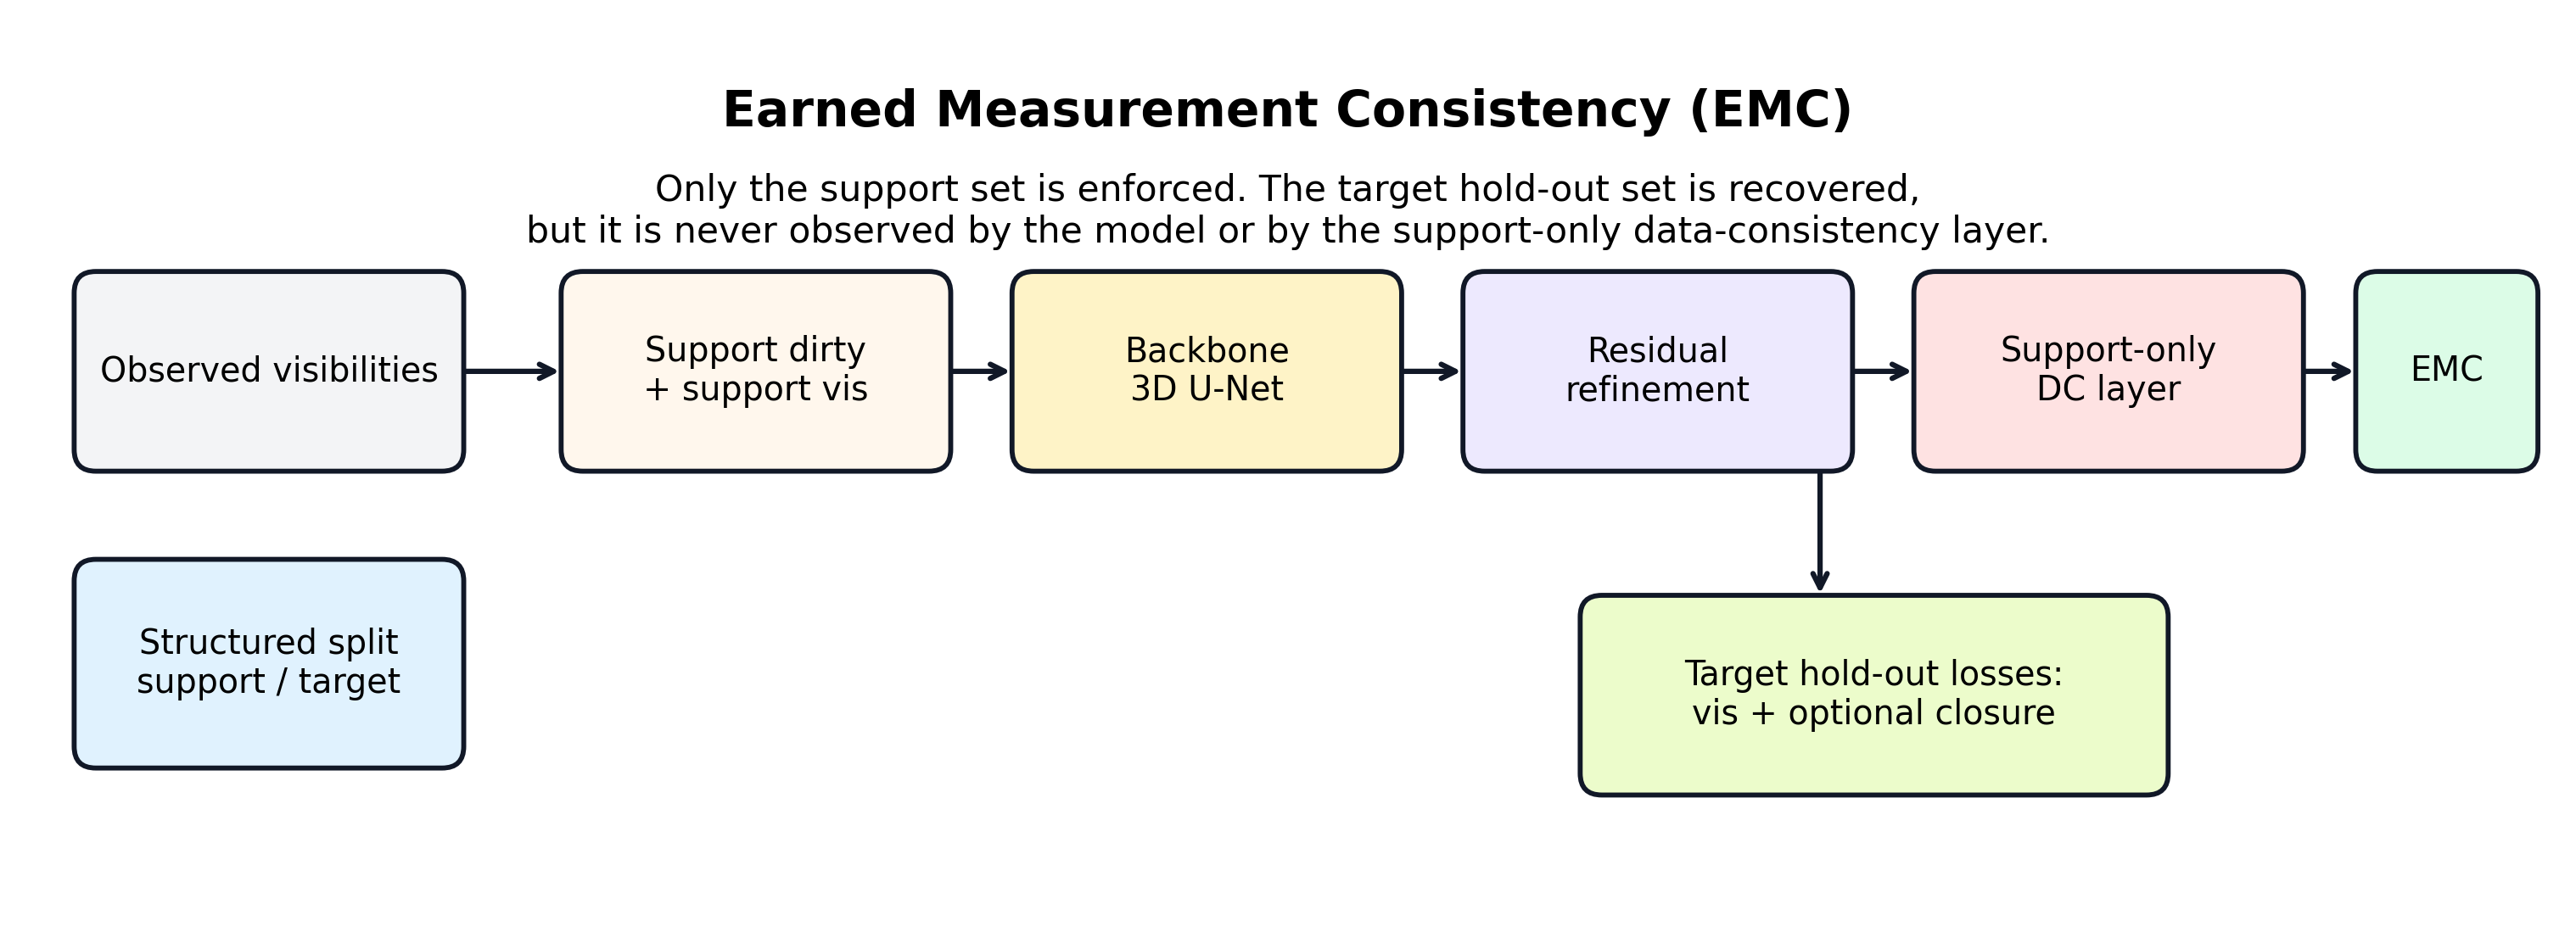
\includegraphics[width=\columnwidth]{figures/fig01_emc_schematic.png}
\caption{Benchmark question and EMC reference implementation. Observed measurements are split deterministically into support and target sets, the model and the support-set data-consistency layer see only the support set, and held-out recovery on the target set becomes the main benchmark quantity.}
\label{fig:emc-schematic}
\end{figure}

\subsection{Synthetic, realism-oriented, and public evaluation paths}

The central synthetic benchmark uses a shared default64 split and reports dirty reconstruction, Tikhonov refinement, the baseline 3D U-Net, residual refinement, CCRR, and EMC. A challenge-inspired realism track adds public-style corruption families already present in the framework: station-track sampling, scan gaps, gain corruption, and baseline-dependent noise heterogeneity.

The public benchmark uses four official calibrated-data releases: M87 2017 (2019-D01-01), M87 2018 (2024-D01-01), 3C279 2017 (2020-D01-01), and Centaurus A 2017 (2021-D03-01). Each release is evaluated under the baseline-track family and under a matched station-dropout sensitivity cohort on a common \(64\times64\) grid. A frozen eht-imaging bridge comparator is scored with the same held-out evaluator as the learned methods.

For real data only, we additionally evaluate a benchmark-legal test-time optimization (TTO) path. TTO adapts EMC on support measurements alone before final prediction, without exposing held-out target data at inference. Synthetic experiments keep this path disabled.

\section{Results}

\subsection{Synthetic benchmark breadth}

Figure~\ref{fig:benchmark-breadth} and Table~\ref{tab:benchmark-matrix} are the quantitative core of the paper. On the released default64 breadth matrix, EMC gives the lowest learned held-out visibility RMSE in all 12 family-support cells. The pooled paired-bootstrap summary is strong in the same snapshot: across 768 paired cases, EMC improves mean held-out visibility RMSE by \(+0.02664\) against CCRR, \(+0.02397\) against residual refinement, and \(+0.02804\) against the baseline 3D U-Net, with all 95 per cent confidence intervals strictly positive.

\begin{figure}
\centering
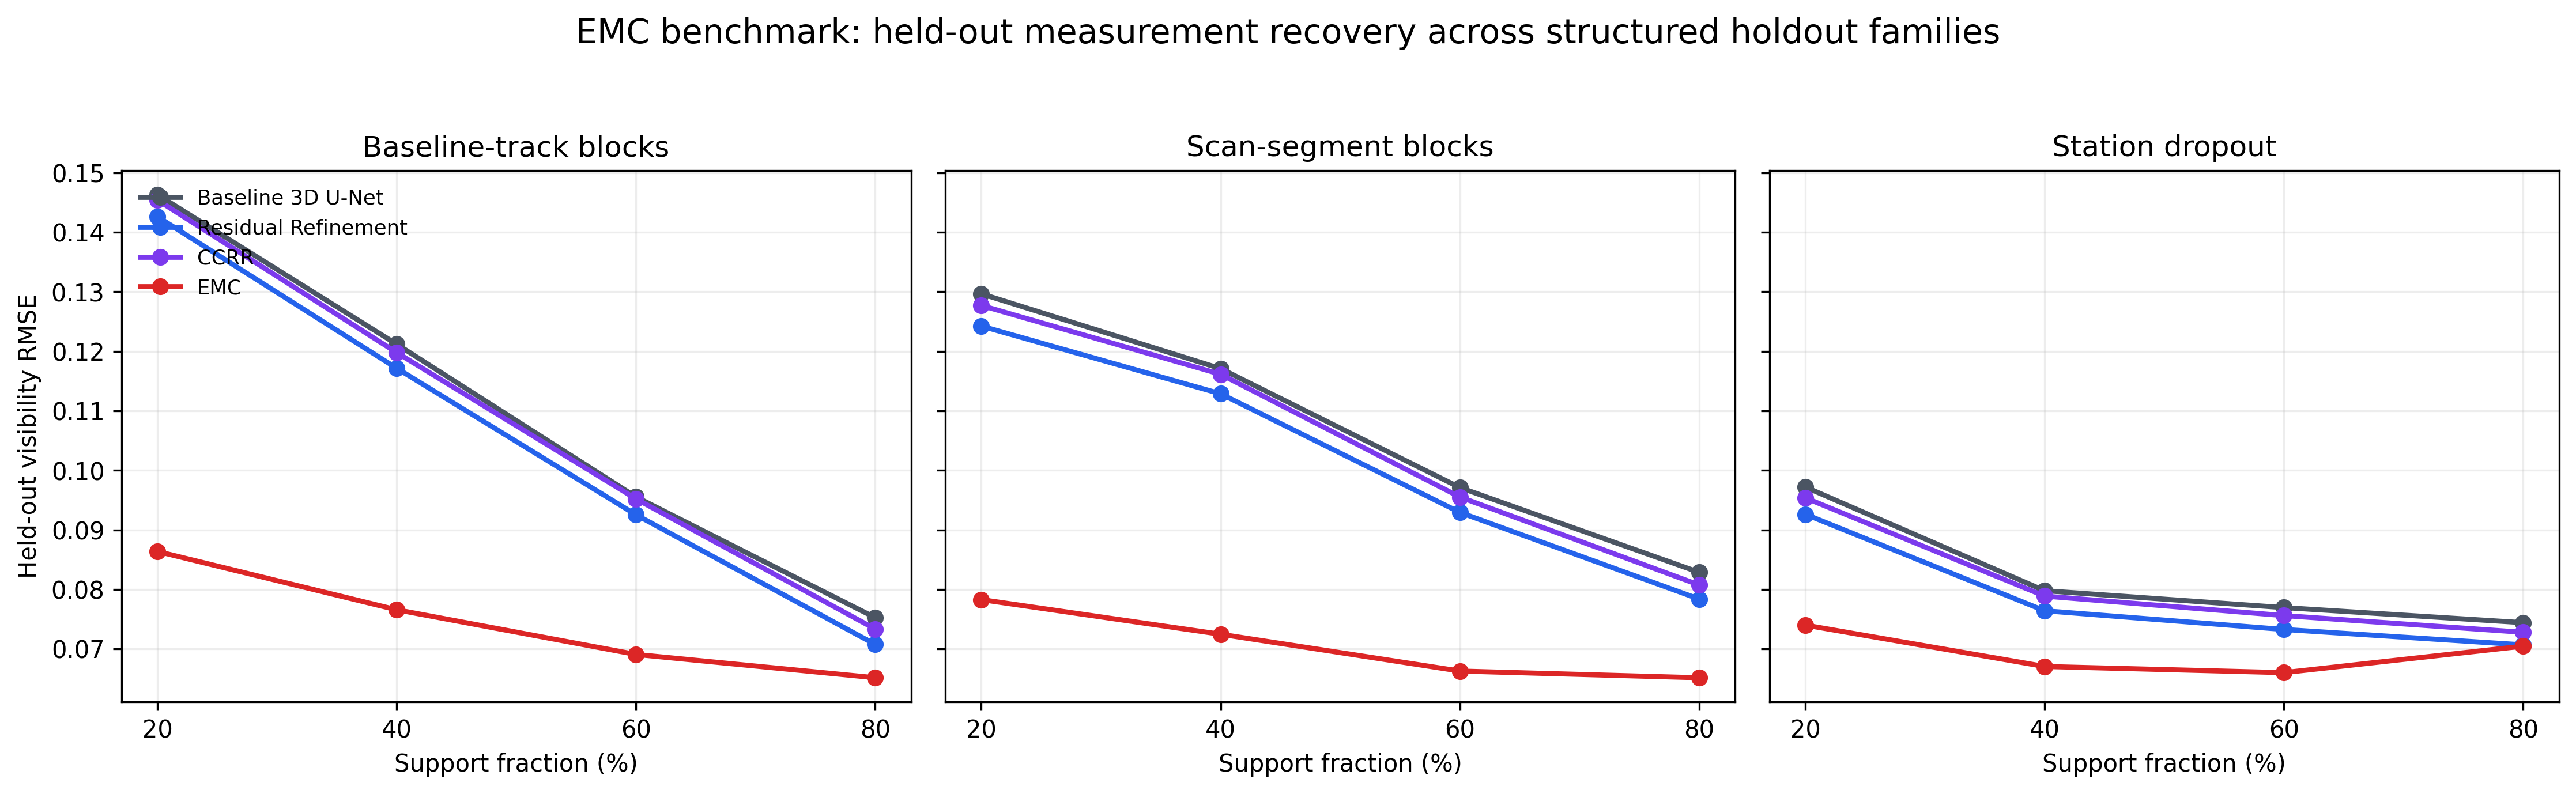
\includegraphics[width=\columnwidth]{figures/fig02_emc_benchmark_support_curve.png}
\caption{Default64 benchmark breadth across the three structured holdout families. The released breadth matrix favors EMC on held-out visibility RMSE throughout the support sweep, but this figure should be read together with the five-seed robustness study rather than as a universal architecture ranking.}
\label{fig:benchmark-breadth}
\end{figure}

\begin{table*}
\centering
\caption{Default64 synthetic benchmark matrix across the three structured holdout families and four support fractions. Lower held-out visibility RMSE is better. DPS is rerun only on the central baseline-track family in this add-on cycle, while EMC conformal UQ is reported as 90 per cent empirical coverage and mean interval width (MIW).}
\label{tab:benchmark-matrix}
\scriptsize
\setlength{\tabcolsep}{4pt}
\begin{tabular}{llccccccc}
\toprule
Holdout family & Support (\%) & EMC & Baseline & Residual & CCRR & DPS & EMC 90\% cov. & EMC MIW \\
\midrule
Baseline-track blocks & 20 & 0.086372 & 0.146334 & 0.142640 & 0.145439 & 0.146634 & 0.853 & 0.161246 \\
Baseline-track blocks & 40 & 0.076572 & 0.121202 & 0.117163 & 0.119797 & 0.143784 & 0.856 & 0.162038 \\
Baseline-track blocks & 60 & 0.069065 & 0.095539 & 0.092545 & 0.095215 & 0.137777 & 0.858 & 0.164417 \\
Baseline-track blocks & 80 & 0.065157 & 0.075252 & 0.070749 & 0.073335 & 0.130919 & 0.870 & 0.184098 \\
Scan-segment blocks & 20 & 0.078278 & 0.129664 & 0.124240 & 0.127704 & n/a & 0.866 & 0.161246 \\
Scan-segment blocks & 40 & 0.072459 & 0.117096 & 0.112871 & 0.116147 & n/a & 0.865 & 0.162038 \\
Scan-segment blocks & 60 & 0.066277 & 0.097107 & 0.092932 & 0.095518 & n/a & 0.864 & 0.164417 \\
Scan-segment blocks & 80 & 0.065148 & 0.082861 & 0.078372 & 0.080735 & n/a & 0.875 & 0.184098 \\
Station dropout & 20 & 0.073993 & 0.097193 & 0.092621 & 0.095378 & n/a & 0.845 & 0.161246 \\
Station dropout & 40 & 0.067045 & 0.079776 & 0.076406 & 0.078876 & n/a & 0.845 & 0.162038 \\
Station dropout & 60 & 0.066009 & 0.076937 & 0.073261 & 0.075594 & n/a & 0.846 & 0.164417 \\
Station dropout & 80 & 0.070459 & 0.074405 & 0.070672 & 0.072785 & n/a & 0.853 & 0.184098 \\
\bottomrule
\end{tabular}
\end{table*}


That favorable matrix is nevertheless only one part of the final story. The bounded five-seed default64 baseline-track study in Table~\ref{tab:seed-robustness} shows that the single-matrix learned ordering is not uniformly seed stable. Averaged over seeds \(7,19,31,42,137\), residual refinement achieves the lowest mean held-out visibility RMSE at every support fraction. The pooled five-seed paired comparison yields a mean delta of \(-0.00644\) for EMC versus residual refinement, with 95 per cent interval \([-0.00689,-0.00600]\). That negative result makes the paper more credible, not less: the benchmark remains useful precisely because it separates a strong released breadth matrix from a stricter robustness check.

The astronomy-facing interpretation is clearest in the sparsest central slice. At 20 per cent support, EMC reduces held-out visibility-error power by \(63.3\) per cent relative to residual refinement, the strongest enforced learned comparator in that slice. As a public-geometry anchor rather than a synthetic-grid unit claim, the matched baseline-track target masks at the closest sparse-support public-EHT regime span roughly \(3.3\)---\(7.8\)\,G$\lambda$ across the central withheld-baseline distribution. Those are the scales that carry the shadow-diameter and brightness-asymmetry information on which dynamic black-hole movie claims depend.

\subsection{Challenge-inspired realism}

The realism-oriented synthetic track remains favorable to EMC. Figure~\ref{fig:realism-track} shows that EMC gives the lowest held-out visibility RMSE across the support sweep, improving from \(0.1802\) to \(0.1293\) relative to CCRR at 20 per cent support and from \(0.1096\) to \(0.1048\) at 80 per cent support. Residual refinement remains structurally stronger on SSIM at the two highest support fractions, so the morphology-versus-measurement trade-off persists even in this harder regime.

\begin{figure}
\centering
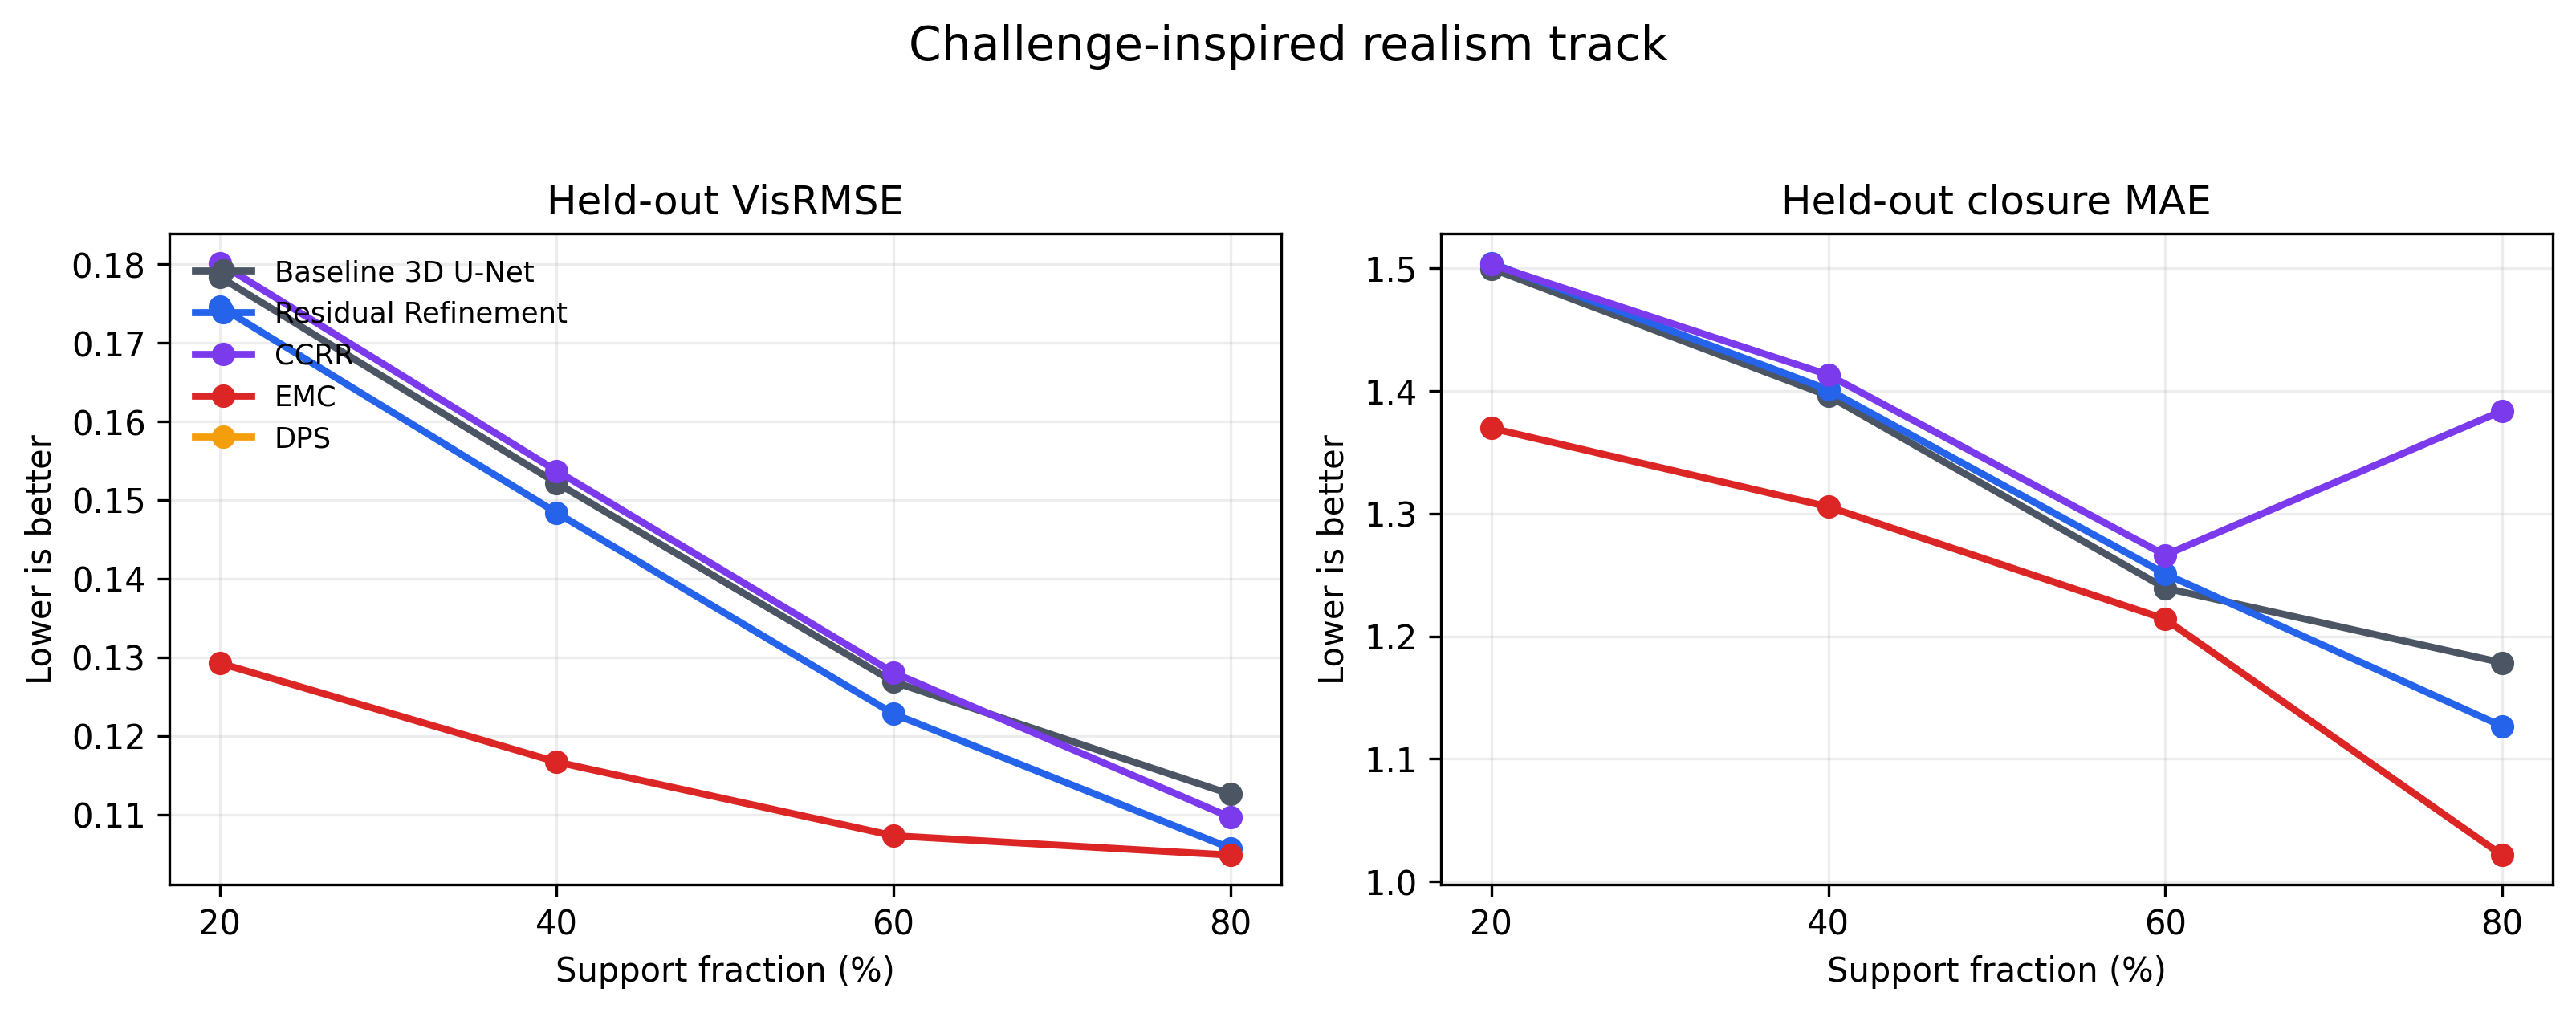
\includegraphics[width=\columnwidth]{figures/fig03_emc_challenge_inspired_realism.png}
\caption{Challenge-inspired realism track built from public-style corruption families already implemented in the repository. EMC remains strongest on held-out visibility RMSE across the support sweep, while residual refinement regains the highest SSIM at higher support fractions.}
\label{fig:realism-track}
\end{figure}

\subsection{Public EHT benchmark and the effect of domain adaptation}

The public-EHT suite should be read as a controlled measurement-domain reality check, not as image-domain validation. Figure~\ref{fig:public-suite} and Table~\ref{tab:public-release-means} summarize the release-level baseline-track picture. TTO materially improves EMC on M87 2017 (\(+0.0696\) held-out-visibility uplift) and especially on 3C279 2017 (\(+0.2275\)), but it degrades M87 2018 (\(-0.0833\)) and Centaurus A 2017 (\(-0.1862\)). On release-average baseline-track means, EMC-TTO is the best model only on 3C279 2017. It therefore does \emph{not} satisfy a broad ``wins on at least two releases'' story.

\begin{figure}
\centering
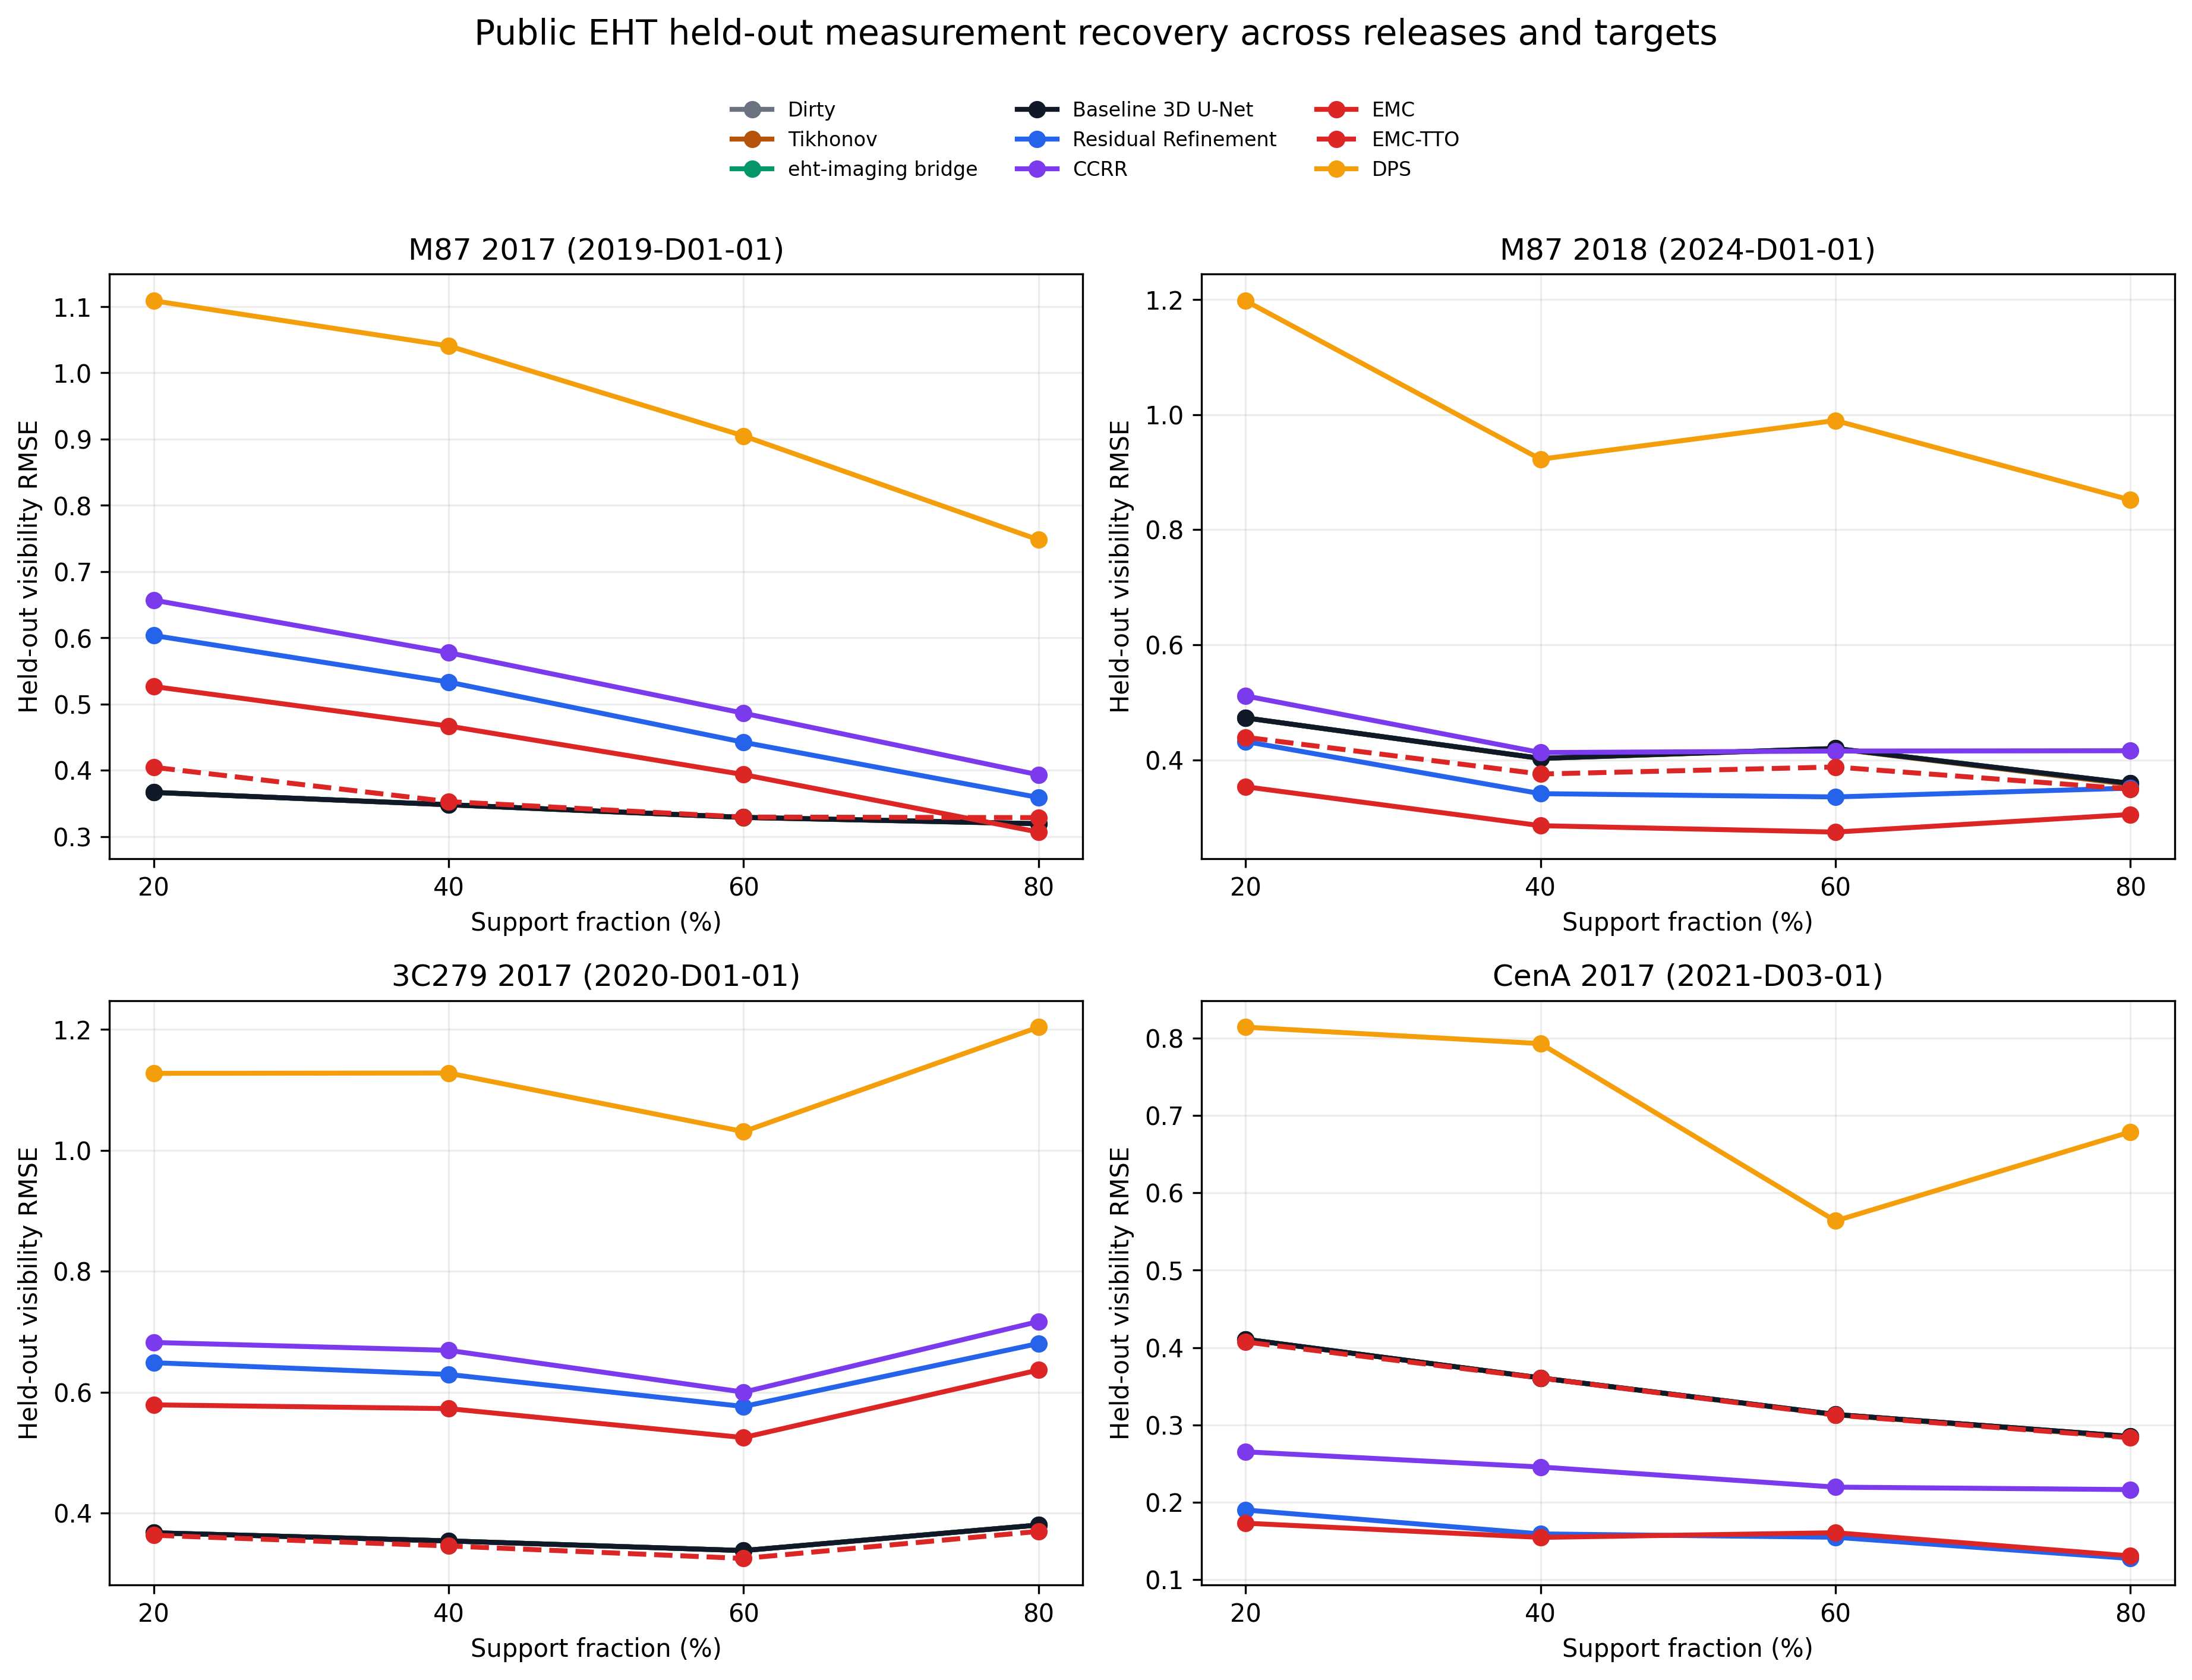
\includegraphics[width=\columnwidth]{figures/fig06_emc_public_eht_suite.png}
\caption{Release-aware public-EHT benchmark. The curves are observation-domain only and should be interpreted as held-out measurement recovery on released data products, not as morphology validation. TTO helps substantially on 3C279 2017, helps modestly on M87 2017, and degrades M87 2018 and Centaurus A 2017.}
\label{fig:public-suite}
\end{figure}

\begin{table*}
\centering
\caption{Release-level public-EHT baseline-track summary with TTO, DPS, and conformal MIW. Positive TTO uplift means lower held-out visibility RMSE than plain EMC. Public UQ reports MIW only because image-domain ground truth is unavailable.}
\label{tab:public-release-means}
\scriptsize
\setlength{\tabcolsep}{4pt}
\resizebox{\textwidth}{!}{%
\begin{tabular}{lccccccccc}
\toprule
Track & Samples & EMC mean & EMC-TTO mean & DPS mean & TTO uplift & EMC MIW & EMC-TTO MIW & Best baseline-track model & Best mean \\
\midrule
3C279 2017 (2020-D01-01) & 8 & 0.578206 & 0.350670 & 1.122637 & +0.227536 & 0.167950 & 0.167950 & EMC-TTO & 0.350670 \\
CenA 2017 (2021-D03-01) & 2 & 0.154797 & 0.341005 & 0.712366 & -0.186207 & 0.167950 & 0.167950 & EMC & 0.154797 \\
M87 2017 (2019-D01-01) & 8 & 0.423486 & 0.353922 & 0.950601 & +0.069564 & 0.167950 & 0.167950 & Tikhonov & 0.340711 \\
M87 2018 (2024-D01-01) & 12 & 0.304620 & 0.387885 & 0.990307 & -0.083265 & 0.167950 & 0.167950 & Standalone Visibility & 0.304567 \\
\bottomrule
\end{tabular}
}
\end{table*}


Release heterogeneity is therefore not a nuisance detail; it is the scientific point. Table~\ref{tab:public-family-robustness} shows that the public story changes across releases and split families. M87 2017 benefits from TTO but still favors Tikhonov on baseline-track mean. M87 2018 is already the most EMC-friendly release without TTO and becomes worse under adaptation. 3C279 2017 is the clearest positive transfer case, with EMC-TTO winning both public families. Centaurus A 2017 remains a small-sample regime in which plain EMC is competitive but TTO is harmful.

\begin{table*}
\centering
\caption{Release-level robustness across the public baseline-track and station-dropout families. Positive family gaps mean the station-dropout split is harder than the corresponding baseline-track split for that method.}
\label{tab:public-family-robustness}
\scriptsize
\setlength{\tabcolsep}{4pt}
\resizebox{\textwidth}{!}{%
\begin{tabular}{lcccccccc}
\toprule
Track & EMC base & EMC-TTO base & EMC station & EMC-TTO station & EMC gap & EMC-TTO gap & Best baseline-track & Best station-dropout \\
\midrule
M87 2017 (2019-D01-01) & 0.423486 & 0.353922 & 0.445604 & 0.333357 & +0.022119 & -0.020565 & Tikhonov & Dirty \\
M87 2018 (2024-D01-01) & 0.304620 & 0.387885 & 0.278218 & 0.373554 & -0.026401 & -0.014331 & Standalone Visibility & Standalone Visibility \\
3C279 2017 (2020-D01-01) & 0.578206 & 0.350670 & 0.482198 & 0.320469 & -0.096007 & -0.030201 & EMC-TTO & EMC-TTO \\
CenA 2017 (2021-D03-01) & 0.154797 & 0.341005 & 0.197272 & 0.440372 & +0.042475 & +0.099367 & EMC & Residual Refinement \\
\bottomrule
\end{tabular}
}
\end{table*}


The pooled public statistics tell a similarly cautious story. On the pooled baseline-track suite, TTO reduces the EMC mean from \(0.3993\) to \(0.3658\), but the paired-bootstrap delta versus plain EMC has 95 per cent interval \([-0.0034,0.0719]\) and \(p=0.0825\), so the pooled improvement is suggestive rather than decisive. TTO is clearly better than CCRR and residual refinement on the same pooled baseline-track suite, and it comes close to parity with the baseline 3D U-Net, the eht-imaging bridge, and Tikhonov without clearly surpassing them. On the pooled station-dropout suite, TTO again improves the EMC mean and is significantly better than the baseline 3D U-Net, the eht-imaging bridge, and Tikhonov.

\begin{center}
\captionof{table}{Selected pooled public-EHT bootstrap comparisons. Positive mean deltas mean the candidate method has lower held-out visibility RMSE than the reference method.}
\label{tab:public-bootstrap}
\scriptsize
\setlength{\tabcolsep}{4pt}
\resizebox{\columnwidth}{!}{%
\begin{tabular}{llccc}
\toprule
Cohort & Comparison & Mean delta & 95\% CI & $p$-value \\
\midrule
Baseline-track & EMC-TTO vs EMC & +0.033507 & [-0.003409, 0.071913] & 0.0825 \\
Baseline-track & EMC-TTO vs Residual Refinement & +0.088892 & [0.052414, 0.127293] & 0.0000 \\
Baseline-track & EMC-TTO vs Baseline 3D U-Net & +0.009323 & [-0.000319, 0.019758] & 0.0659 \\
Baseline-track & EMC-TTO vs eht-imaging bridge & +0.009307 & [-0.000337, 0.019731] & 0.0664 \\
Baseline-track & EMC-TTO vs Tikhonov & +0.009000 & [-0.000652, 0.019446] & 0.0776 \\
Station-dropout & EMC-TTO vs EMC & +0.018720 & [-0.018835, 0.055916] & 0.3169 \\
Station-dropout & EMC-TTO vs Baseline 3D U-Net & +0.016369 & [0.006413, 0.027238] & 0.0024 \\
Station-dropout & EMC-TTO vs eht-imaging bridge & +0.016370 & [0.006417, 0.027239] & 0.0024 \\
Station-dropout & EMC-TTO vs Tikhonov & +0.016369 & [0.006409, 0.027245] & 0.0024 \\
\bottomrule
\end{tabular}
}
\end{center}


\subsection{Synthetic-to-public transfer gap}

Figure~\ref{fig:transfer-gap} sharpens the paper's final interpretation. The left panel summarizes the strong synthetic breadth advantage of EMC over the learned comparators on held-out visibility RMSE. The public panels and release summaries show something different: the synthetic gain does not transfer uniformly, and the sign and magnitude of the gap vary by release. That heterogeneity strengthens the benchmark contribution because it shows that earned-versus-enforced evaluation continues to separate regimes once released measurements are introduced.

\begin{figure}
\centering
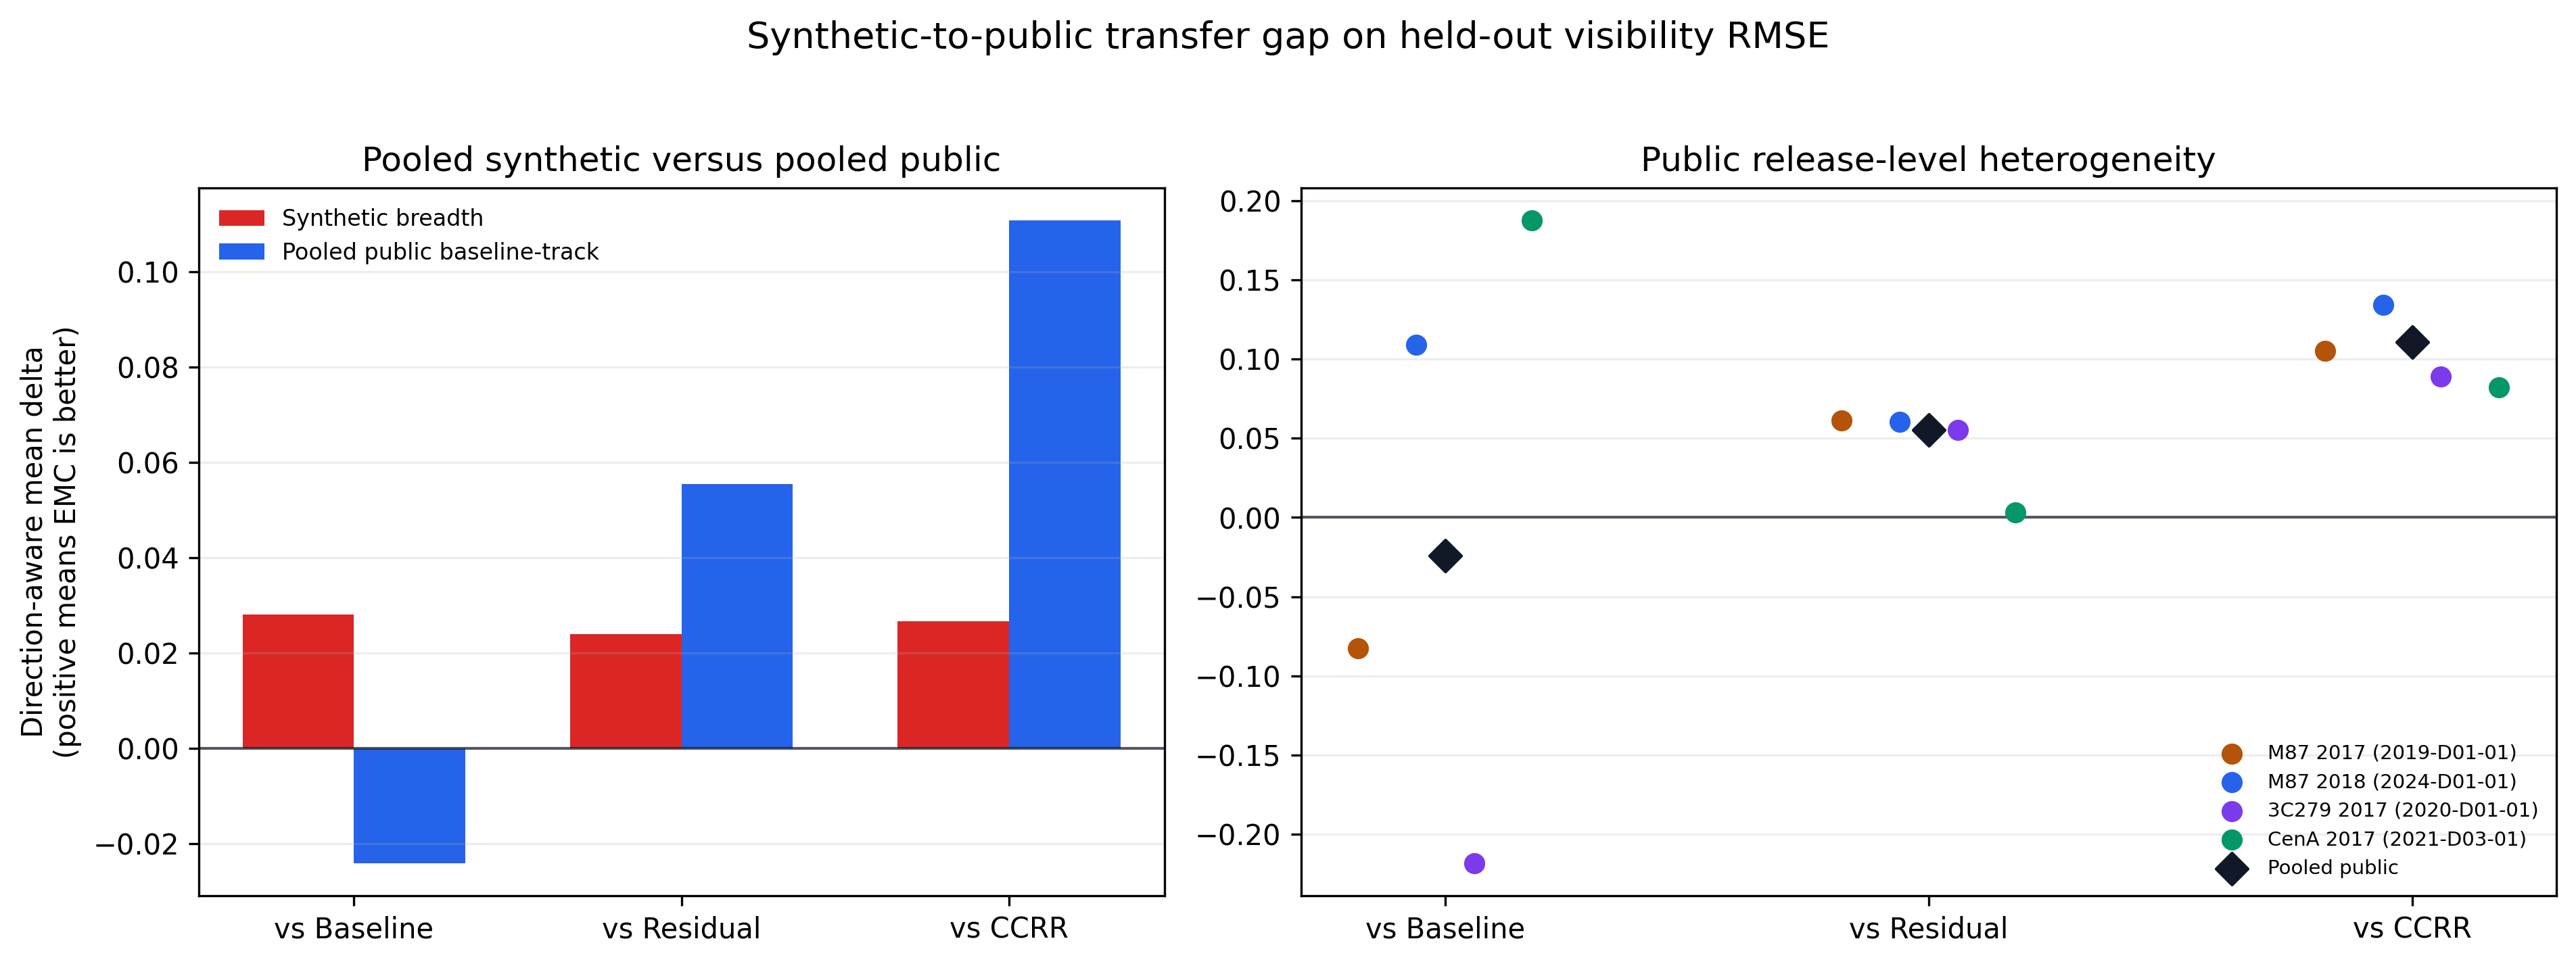
\includegraphics[width=\columnwidth]{figures/fig07_emc_public_transfer_gap.png}
\caption{Synthetic-to-public transfer gap on held-out visibility RMSE. The synthetic breadth result is clearly favorable to EMC in the released default64 matrix, while the public release-level deltas are heterogeneous and partly reversed. Positive values mean the candidate method is better.}
\label{fig:transfer-gap}
\end{figure}

\begin{figure}
\centering
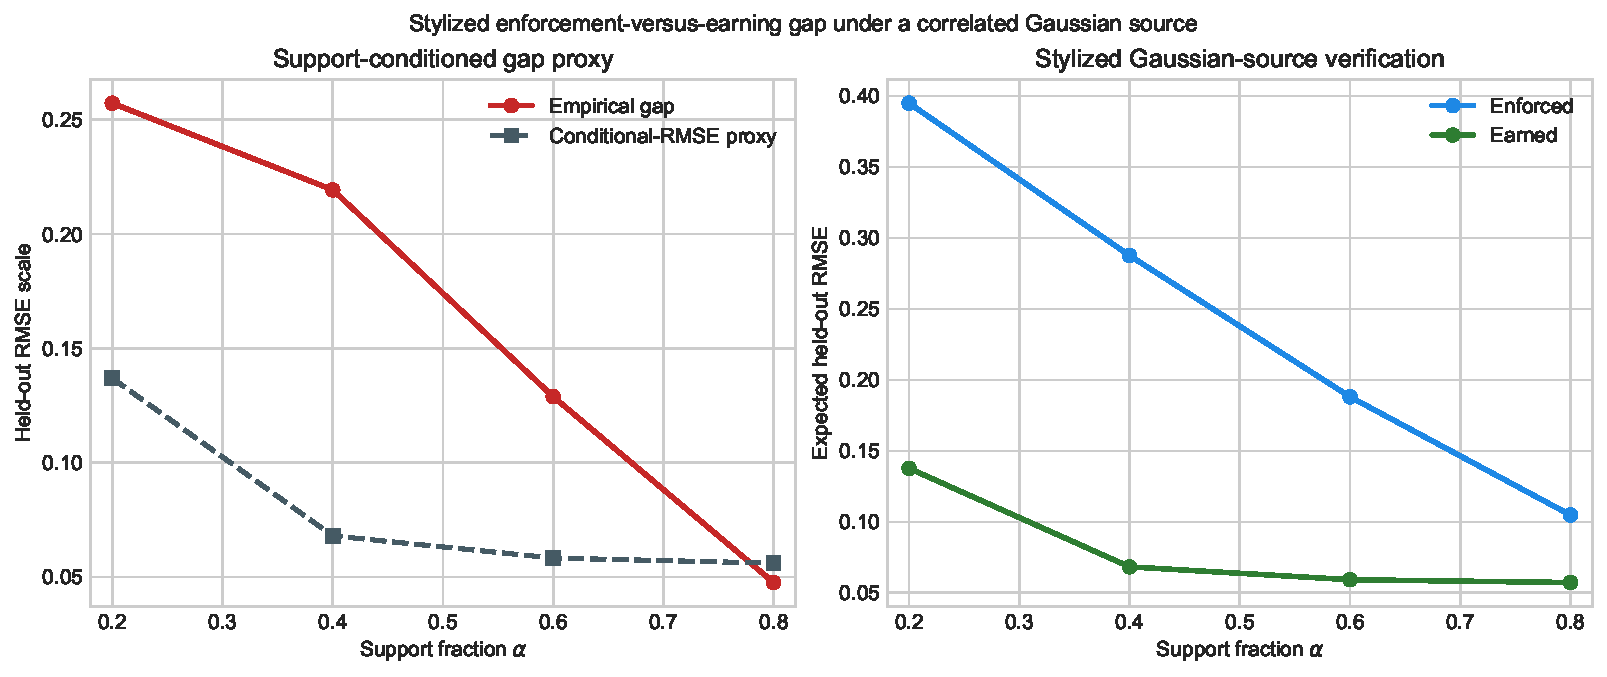
\includegraphics[width=\columnwidth]{figures/fig06_consistency_bound.pdf}
\caption{Numerical verification of the stylized enforcement-versus-earning gap. In the linear-Gaussian toy setting, the empirical gap shrinks as the support fraction \(\alpha\) increases, tracking the decline in the conditional-RMSE proxy derived from the support-conditioned target covariance.}
\label{fig:consistency-bound}
\end{figure}

\begin{center}
\captionof{table}{Bounded five-seed robustness study on the default64 baseline-track family. Means and population standard deviations are computed over seeds 7, 19, 31, 42, and 137. Lower held-out visibility RMSE is better.}
\label{tab:seed-robustness}
\scriptsize
\setlength{\tabcolsep}{5pt}
\resizebox{\columnwidth}{!}{%
\begin{tabular}{lccccc}
\toprule
Support (\%) & EMC mean $\pm$ std & Residual mean $\pm$ std & CCRR mean $\pm$ std & Baseline mean $\pm$ std & Best mean model \\
\midrule
80 & 0.115676 $\pm$ 0.006969 & 0.109503 $\pm$ 0.006575 & 0.116167 $\pm$ 0.005156 & 0.115504 $\pm$ 0.003861 & Residual Refinement \\
60 & 0.117839 $\pm$ 0.007454 & 0.111488 $\pm$ 0.007928 & 0.119436 $\pm$ 0.006325 & 0.119051 $\pm$ 0.004628 & Residual Refinement \\
40 & 0.119454 $\pm$ 0.007485 & 0.112935 $\pm$ 0.008682 & 0.121751 $\pm$ 0.006494 & 0.121440 $\pm$ 0.004955 & Residual Refinement \\
20 & 0.120329 $\pm$ 0.007614 & 0.113592 $\pm$ 0.009633 & 0.122879 $\pm$ 0.006917 & 0.122689 $\pm$ 0.005324 & Residual Refinement \\
\bottomrule
\end{tabular}
}
\end{center}


Figure~\ref{fig:qualitative} is retained only as secondary visual evidence after the quantitative core. The synthetic panel visualizes the benchmark regime with image-domain ground truth, whereas the public panel remains observation-domain only and is included solely to make the release-aware evaluation pipeline concrete.

\begin{figure}[t]
\centering
\begin{subfigure}[t]{0.49\columnwidth}
  \centering
  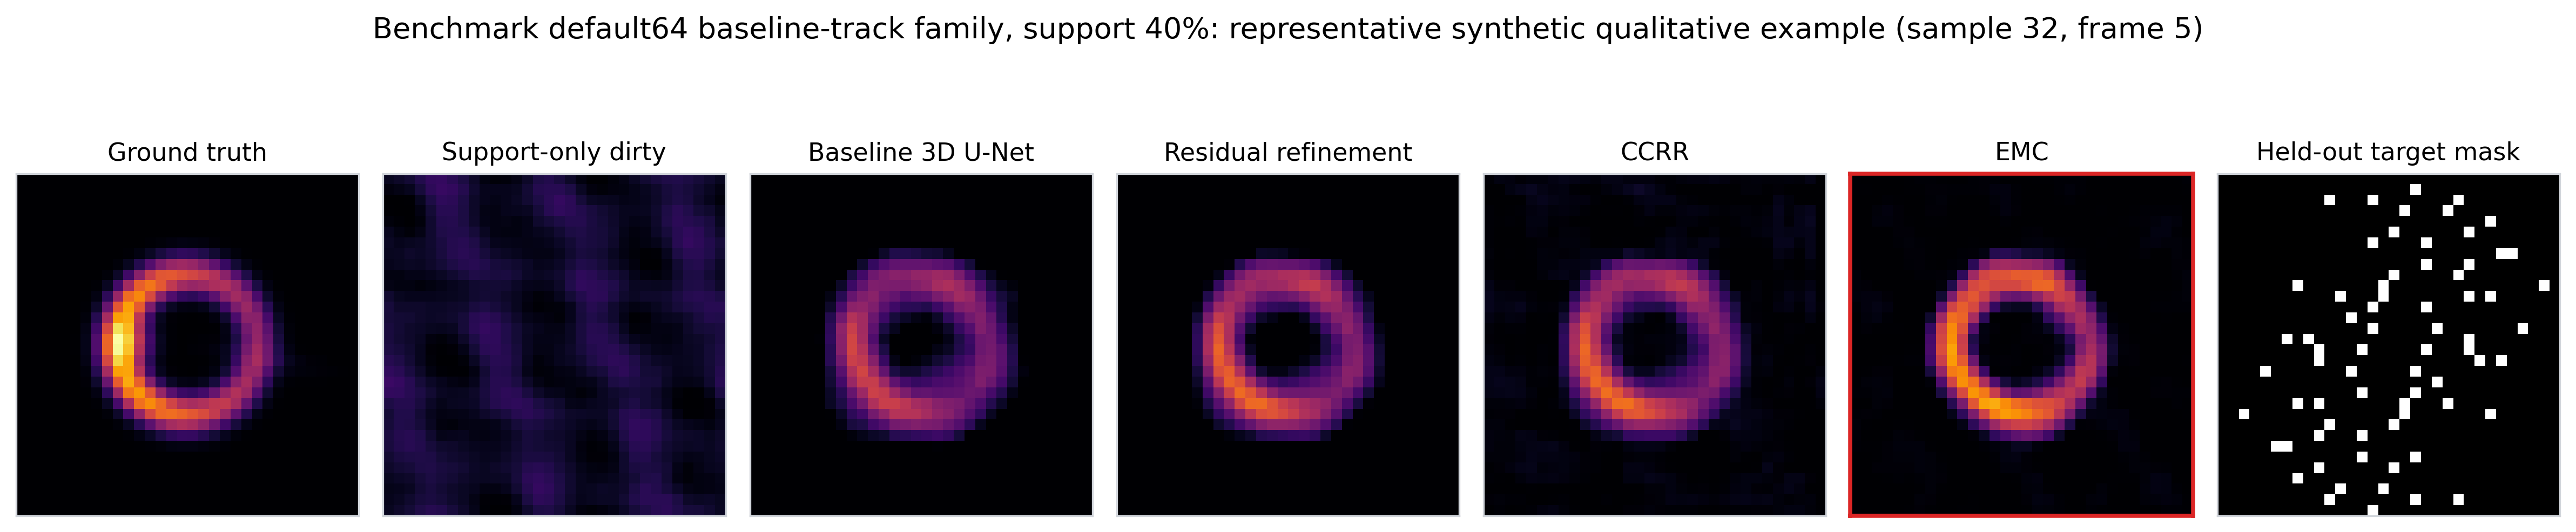
\includegraphics[width=\linewidth]{figures/fig08_emc_synthetic_qualitative.png}
  \caption{Representative synthetic default64 baseline-track example at 40 per cent support.}
\end{subfigure}
\hfill
\begin{subfigure}[t]{0.49\columnwidth}
  \centering
  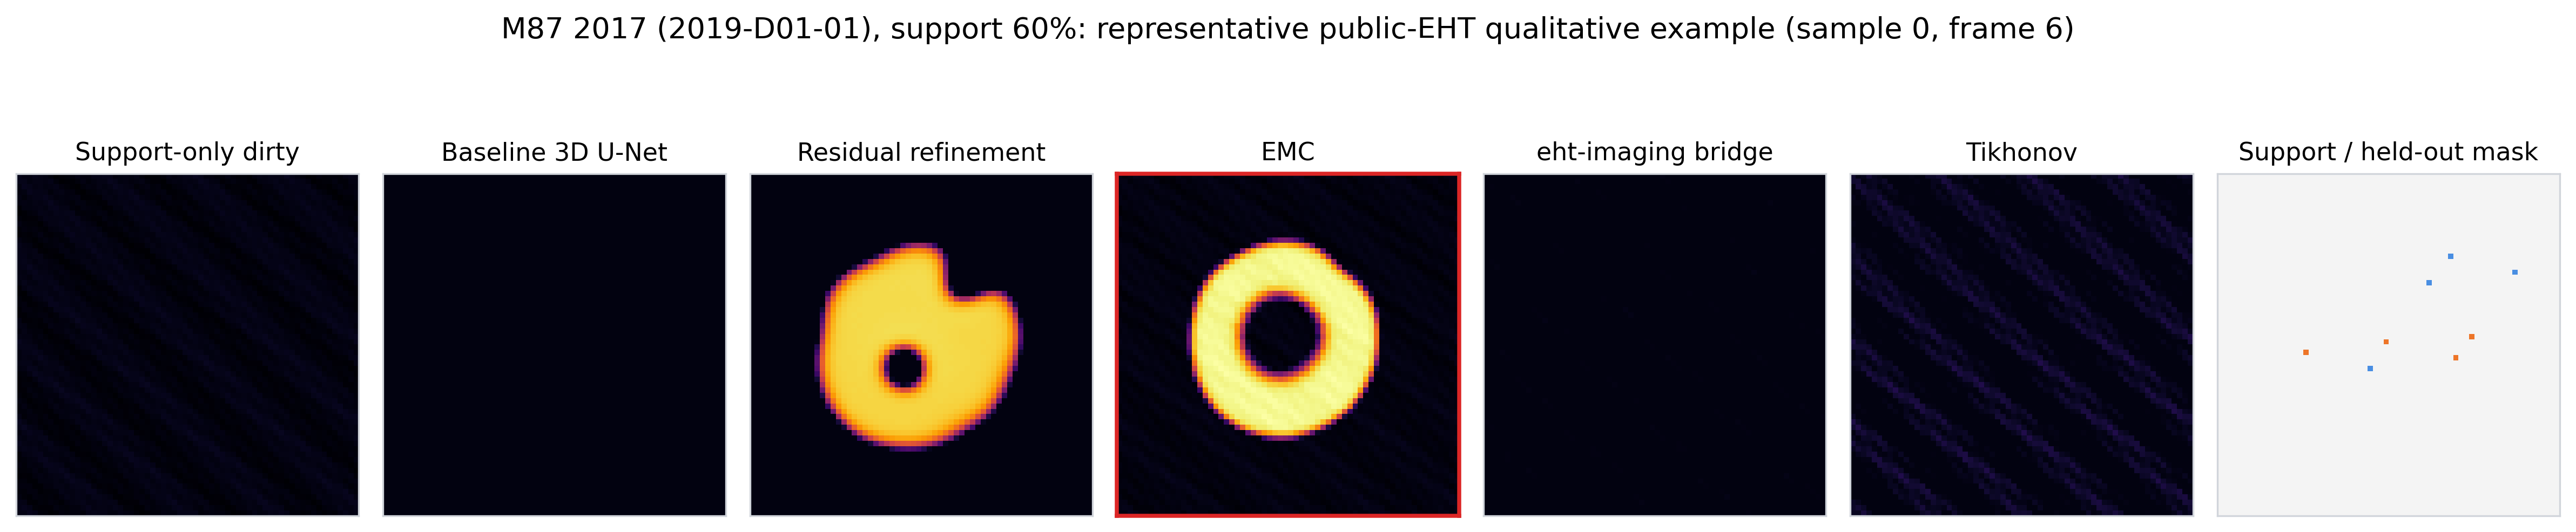
\includegraphics[width=\linewidth]{figures/fig09_public_eht_qualitative.png}
  \caption{Representative public-EHT example chosen by the documented pooled-median rule.}
\end{subfigure}
\caption{Qualitative panels as secondary evidence only. The synthetic panel helps visualize the benchmark regime with ground truth; the public panel is observation-domain only and is not used to make morphology claims.}
\label{fig:qualitative}
\end{figure}

\section{Discussion}

The strongest final signal from this study is benchmark-oriented rather than method-oriented. The released default64 breadth matrix favors EMC strongly, and the realism-oriented synthetic track remains supportive. But the five-seed baseline-track study shows that a central learned-method ordering can change once seed robustness is brought into view. Public-EHT validation is likewise mixed by release, split family, and comparator.

That combination of results is scientifically useful. It shows that support-target evaluation can reveal held-out measurement recovery that is not reducible to support-set enforcement, but it also shows that no compact learned reference implementation should be treated as universally dominant on the basis of one favorable benchmark slice. In practice, the benchmark now distinguishes three things that are often conflated: released synthetic breadth, seed robustness on the core family, and transfer to released public measurements.

For ngEHT science, that distinction matters directly. Learned methods trained with earned-consistency objectives are better positioned for dynamic black-hole movie generation than methods relying only on enforced consistency, because movie generation requires extrapolation to unobserved time steps and unobserved coefficients --- exactly the target-holdout regime that the benchmark isolates. A benchmark that cannot separate those behaviors would be poorly aligned with the scientific use case that motivates dynamic VLBI in the first place.

The domain-adaptation results sharpen the same point. TTO partially closes the synthetic-to-public gap, especially on 3C279 2017 and to a lesser degree on M87 2017. The remaining gap on M87 2018 and Centaurus A 2017 points to a scientifically interesting question: what properties of particular release products, day-band mixes, or calibration structures make certain public tracks easier or harder to generalize to? Exposing that heterogeneity is itself a useful contribution of the benchmark.

The TTO procedure also adds inference-time compute. In the current implementation it performs 50 support-only adaptation steps per sample. That is acceptable for scientific imaging, where latency is not the primary constraint, but it is incompatible with any real-time use case.

The benchmark protocol is not specific to VLBI.
Cardiac cine MRI shares the same mathematical structure:
a time-varying source observed via undersampled Fourier
measurements with structured missingness patterns.
The earned-versus-enforced distinction applies directly ---
methods that enforce k-space consistency at observed
frequencies do not necessarily generalize to unobserved
frequencies across cardiac phases. A benchmark analogous
to the one presented here, applied to the FastMRI cine
dataset, would test the same protocol in a domain where
ground truth is available and the clinical stakes are
higher. We leave this cross-domain extension to future work.

Taken together, the astronomy-facing and cross-domain readings point in the same direction. The value of the benchmark is not that it guarantees one compact learned method will dominate every regime, but that it makes the extrapolation problem itself measurable in settings where structured Fourier missingness is the scientific bottleneck.

\section{Limitations}

The synthetic and challenge-inspired tracks remain VLBI-inspired rather than telescope-accurate end-to-end simulations. The public suite is broader than a single sanity check, but it is still observation-domain only and does not provide image-domain ground truth. The eht-imaging bridge is a frozen benchmark-stable external comparator rather than a fully tuned astronomy pipeline under each release's natural operating envelope.

The TTO procedure also adds inference-time compute. In the current implementation it performs 50 support-only adaptation steps per sample. That is acceptable for scientific imaging, where latency is not the primary constraint, but it is incompatible with any real-time use case.

Finally, the current default64 paper does not include a fully rerun ablation suite at the same resolution. The main benchmark, public suite, realism track, theory figure, and five-seed robustness study are all current and reproducible; the next natural extension would be a matched default64 ablation pass if one wanted to turn the reference implementation itself into a larger method paper.

\section{Conclusion}

We present a reproducible $64\times64$ benchmark for earned versus enforced measurement consistency in dynamic VLBI-style inference, together with a compact reference implementation, a stylized theoretical motivation, and controlled public-EHT measurement-domain validation. The synthetic breadth matrix is strong and the realism-oriented track remains favorable to EMC, but the five-seed robustness study and the mixed public-transfer results narrow the right scientific claim.

The clearest signal from this study is not which method wins, but that the earned-versus-enforced distinction is scientifically meaningful at all scales --- synthetic, domain-adapted, and released. A benchmark that exposes that distinction, with deterministic manifests, paired-bootstrap reporting, release-aware public evaluation, and a concrete reference implementation, is the paper's primary contribution.

\section*{Acknowledgements}

The authors thank the Event Horizon Telescope Collaboration for releasing the official calibrated data products used in the public validation suite, and acknowledge the open scientific Python ecosystem that supported the computational work reported here.

\section*{Data Availability}

The repository snapshot accompanying this manuscript includes the code, resolved configuration files, deterministic split manifests, benchmark output manifests, and artifact-generation scripts used in the study. The current paper-facing outputs are distributed under \texttt{outputs/emc\_benchmark\_artifacts}, \texttt{outputs/public\_eht\_suite\_artifacts}, \texttt{outputs/emc\_seed\_robustness\_artifacts}, \texttt{outputs/dps\_benchmark\_artifacts}, and \texttt{outputs/emc\_conformal\_uq}, with a reproducibility verification pass recorded by \texttt{scripts/verify\_reproducibility.py}. No new real astronomical observations were acquired for this work. The public validation uses the official Event Horizon Telescope calibrated-data releases \texttt{2019-D01-01} (M87 2017, DOI \href{https://doi.org/10.25739/g85n-f134}{10.25739/g85n-f134}), \texttt{2024-D01-01} (M87 2018, DOI \href{https://doi.org/10.25739/epm5-r371}{10.25739/epm5-r371}), \texttt{2020-D01-01} (3C279 2017, DOI \href{https://doi.org/10.25739/vty0-ve39}{10.25739/vty0-ve39}), and \texttt{2021-D03-01} (Centaurus A 2017, DOI \href{https://doi.org/10.25739/kejs-2n22}{10.25739/kejs-2n22}).

\balance
\bibliographystyle{mnras}
\bibliography{references}

\label{lastpage}
\end{document}
